% -*- coding: utf-8; mode: latex; -*-
%
% FIT2018 向け LaTeX クラスファイル
% https://github.com/trueroad/FITpaper-class
%
% サンプルファイル
%
% Copyright (C) 2018 Masamichi Hosoda.
% All rights reserved.
% 

\documentclass{FITpaper}

% 図の貼り込み用
\usepackage{graphicx}

% 最終ページで両カラムの下端を揃える
\usepackage[balance]{nidanfloat}

% 和文タイトル
\jtitle{FIT2018向け\LaTeX クラスファイルのサンプル}

% 欧文タイトル
\etitle{Sample \LaTeX~Class File for FIT2018}

% 著者数:著者の数だけ c を書く
\authors{cc}

% 和文著者名:著者名間に & を書く
% 所属番号を \affmark でつける
\jauthors{%
  細田 真道\affmark{1} &
  〇〇 〇〇\affmark{2}
}

% 欧文著者名:著者名間に & を書く
\eauthors{%
  Masamichi Hosoda &
  Foo Bar Baz
}

% 所属
% \affmark でつけた番号毎に指定
\afftext{1}{http://www.trueroad.jp}
\afftext{2}{〇〇〇〇〇〇〇〇〇〇〇〇〇〇〇〇〇〇〇〇〇〇〇〇〇〇.
Foo bar baz boo bar baz Laboratories, Foo Corporation.}

\begin{document}

\maketitle

\section{セクション}
\subsection{サブセクション}
\subsubsection{サブサブセクション}

FIT2018第17回情報科学技術フォーラム\cite{fit2018}向けに
\LaTeX で使えるクラスファイル\cite{fitpaper-class}を作ってみました。
Lua\LaTeX 、p\LaTeX 、up\LaTeX に対応しています。
基本的にはサイトに記載のある紙サイズ、ページ設定(マージン等)や、
サイトに掲載されている原稿見本のサンプルファイルFITpaper.docxに
設定されているフォントサイズ、行送り、アキ等と
同様なものを指定しているつもりです。

\section{必要なもの}

\subsection{Lua\LaTeX で使う場合}

\begin{itemize}
\item Lua\LaTeX
\item Lua\TeX -ja
\item jlreq.cls
  \begin{itemize}
  \item 2018/04/11 以降が必要です。
    (それ以前でもパッチ\cite{column_gap}を当てれば恐らく動きます。)
  \end{itemize}
\item 各種フォント
  \begin{itemize}
  \item 源ノ明朝
  \item 源ノ角ゴシック
  \item STIX 2
    \begin{itemize}
    \item \TeX~Live 2017には収録されていないようなので、
      自分でダウンロードしてインストールしておく必要があります。
    \end{itemize}
  \item \TeX~Gyre Heros
  \item \TeX~Gyre Cursor
  \end{itemize}
\end{itemize}

\subsection{p\LaTeX~/ up\LaTeX で使う場合}

作成者は基本的にLua\LaTeX を使っているため、
うまく動かないことがあるかもしれません。

\begin{itemize}
\item p\LaTeX またはup\LaTeX
\item jlreq.cls
  \begin{itemize}
  \item 2018/04/11 以降が必要です。
    (それ以前でもパッチ\cite{column_gap}を当てれば恐らく動きます。)
  \end{itemize}
\item 各種フォント
  \begin{itemize}
  \item newtx
  \item \TeX~Gyre Terms
  \item \TeX~Gyre Heros
  \item \TeX~Gyre Cursor
  \end{itemize}
\end{itemize}

\section{書き方}

ソースファイルの書き方の概要を説明します。
実際の書き方の例は、
本サンプルのソースファイルsample.texや、
著者名が多い場合のサンプルのソースファイルsample2.texをご覧ください。

\subsection{タイトル}

和文タイトルを\texttt{\textbackslash jtitle}で、
欧文タイトルを\texttt{\textbackslash etitle}で指定します。

\subsection{著者}

著者は1段で書くか、人数が多ければ2段に分けて書くことができます。
1段目の著者数を\texttt{\textbackslash authors}で指定します。
これには著者の数だけ\texttt{c}を書きます。
1段目の和文著者名を\texttt{\textbackslash jauthors}で指定します。
複数の著者名間は\texttt{\&}で区切って記述します。
1段目の欧文著者名を\texttt{\textbackslash eauthors}で指定します。
こちらも複数の著者名間を\texttt{\&}で区切って記述します。

著者の人数が多くて2段目が必要であれば、
2段目の著者数、和文著者名、欧文著者名をそれぞれ、
\texttt{\textbackslash authorstwo}
\texttt{\textbackslash jauthorstwo}
\texttt{\textbackslash eauthorstwo}
で1段目と同様に指定します。
これら2段目の指定が無ければ著者は1段のみで出力され、
2段目の指定があれば2段とも出力されます。
2段のサンプルはsample2.texをご覧ください。

\subsection{所属}

和文著者のところで、
各著者名に\texttt{\textbackslash af\mbox{}fmark}で所属番号を付けます。
所属名は所属番号ごとに\texttt{\textbackslash af\mbox{}ftext}で指定します。

FIT2018サイトの原稿見本では所属番号ではなく、
所属記号として$\dag$や$\ddag$が使われていますが、
本クラスファイルでは記号ではなく番号にしています。
これは人名に$\dag$などを付けたくなかったからです。

もしどうしても原稿見本と同様に$\dag$や$\ddag$を使いたいのであれば、
\LaTeX の脚注の仕組みを使っていますので、
\texttt{\textbackslash maketitle}の前に脚注を記号に変更する
\texttt{\textbackslash renewcommand \{
  \textbackslash thefootnote \} \{
  \textbackslash fnsymbol \{ footnote \} \}}
  %\renewcommand{\thefootnote}{\fnsymbol{footnote}}
を入れ、所属番号として2 ($\dag$)と3 ($\ddag$)を使う
ことで実現できます。
詳しくは\LaTeX の参考書などをご覧ください。

\subsection{図表}

図\ref{fig:test}や表\ref{tbl:test}のように出力ができます。
\LaTeX の標準的な書き方で使えます。

図\ref{fig:test}はプリアンブルでgraphicxパッケージを読み込み
figure環境内で\texttt{\textbackslash includegraphics}を
使ってPDFを貼り込みました。
このPDFは楽譜作成プログラムLilyPond\cite{lilypond}で作成したものです。

表\ref{tbl:test}はtable環境内でtabular環境を使ったものです。

\begin{figure}
  \centering
  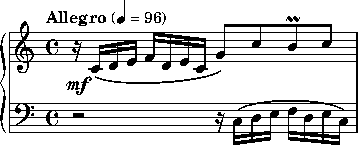
\includegraphics{invention1}
  \caption{テストの図です}
  \label{fig:test}
\end{figure}

\begin{table}
  \centering
  \begin{tabular}{c|cc}
    & 表頭1 & 表頭2 \\
    \hline
    表側1 & 表体A & 表体B \\
    表側2 & 表体C & 表体D \\
  \end{tabular}
  \caption{テストの表です}
  \label{tbl:test}
\end{table}

\subsection{数式}

数式は、式(\ref{eq:test})のように出力できます。

\begin{align}
  \frac{\pi}{2} &=
  \left( \int_{0}^{\infty} \frac{\sin x}{\sqrt{x}} dx \right)^2 \nonumber \\
  &= \sum_{k=0}^{\infty} \frac{(2k)!}{2^{2k}(k!)^2} \frac{1}{2k+1} \nonumber \\
  &= \prod_{k=1}^{\infty} \frac{4k^2}{4k^2 - 1}
  \label{eq:test}
\end{align}

amsmathパッケージを読み込んでいます。
Lua\LaTeX の場合はunicode-mathパッケージも読み込みます。
unicode-mathパッケージを読み込むと、
数式内の書体の指定方法など、一部の使い方が\LaTeX 標準とは異なります。
詳しくはパッケージのドキュメントなどをご覧ください。

\subsection{最終ページで両カラムの下端を揃える}

最終ページでは両カラムの下端を揃えた方がよいでしょう。
揃える方法はいくつかあるようですが、
本サンプルではjlreq.clsのドキュメントに記載されている方法、
つまりプリアンブルでnidanfloatパッケージをbalanceオプション付きで
読み込むことで実現しています。
もう一つのサンプルであるsample2.texや、
デバッグ用テストソースdebug.texではこの処理をしていないため、
これらをコンパイルしたsample2.pdfやdebug.pdfは
最終ページの両カラム下端が揃いません。
詳しくはjlreq.clsのドキュメントおよびnidanfloatパッケージの
ドキュメントをご覧ください。

\subsection{クラスオプション}

クラスでフォント設定しないようにするオプションを用意しています。
別のフォントを指定したい場合に使うとよいでしょう。

\begin{itemize}
\item \texttt{no\_jafont\_settings}
  \begin{itemize}
  \item 和文フォントを設定しません
  \end{itemize}
\item \texttt{no\_lgcfont\_settings}
  \begin{itemize}
  \item 欧文フォントを設定しません
  \end{itemize}
\item \texttt{no\_mathfont\_settings}
  \begin{itemize}
  \item 数式フォントを設定しません
  \item amsmathパッケージやunicode-mathパッケージもロードしません
  \end{itemize}
\end{itemize}

\subsection{脚注}

所属の所で述べたように、所属の出力に脚注の仕組みを使っています。
FITの原稿本文で脚注を使いたくなることは少ないと思いますが、
どうしても使いたい場合には、脚注表記
(\texttt{\textbackslash thefootnote}の設定)を
所属用と本文用で別々のものを設定
(\texttt{\textbackslash maketitle}の前で所属用、後で本文用を設定)し、
本文で脚注を使う前に脚注カウンタをクリアすればよいと思います。
詳しくは\LaTeX の参考書などをご覧ください。

\acknowledgment{%
  謝辞の文章を\texttt{\textbackslash acknowledgment}で指定します。
  使わなければ謝辞は出力されません。
}

\begin{thebibliography}{9}

\bibitem{fit2018}
  FIT2018第17回情報科学技術フォーラム. \\
  https://www.ipsj.or.jp/event/fit/fit2018/index.html
\bibitem{fitpaper-class}
  FIT2018向け\LaTeX クラスファイル. \\
  https://github.com/trueroad/FITpaper-class
\bibitem{column_gap}
  Fix \verb|`column_gap`| class option. \\
  https://github.com/abenori/jlreq/pull/25
\bibitem{lilypond}
  楽譜作成プログラムLilyPond. \\
  http://lilypond.org

\end{thebibliography}

\end{document}
